\let\negmedspace\undefined
\let\negthickspace\undefined
\documentclass[journal]{IEEEtran}
\usepackage[a5paper, margin=10mm, onecolumn]{geometry}
%\usepackage{lmodern} % Ensure lmodern is loaded for pdflatex
\usepackage{tfrupee} % Include tfrupee package

\setlength{\headheight}{1cm} % Set the height of the header box
\setlength{\headsep}{0mm}     % Set the distance between the header box and the top of the text

\usepackage{gvv-book}
\usepackage{gvv}
\usepackage{cite}
\usepackage{amsmath,amssymb,amsfonts,amsthm}
\usepackage{algorithmic}
\usepackage{graphicx}
\usepackage{textcomp}
\usepackage{xcolor}
\usepackage{txfonts}
\usepackage{listings}
\usepackage{enumitem}
\usepackage{mathtools}
\usepackage{gensymb}
\usepackage{comment}
\usepackage[breaklinks=true]{hyperref}
\usepackage{tkz-euclide} 
\usepackage{listings}
% \usepackage{gvv}                                        
\def\inputGnumericTable{}                                 
\usepackage[latin1]{inputenc}                                
\usepackage{color}                                            
\usepackage{array}                                            
\usepackage{longtable}                                       
\usepackage{calc}                                             
\usepackage{multirow}                                         
\usepackage{hhline}                                           
\usepackage{ifthen}                                           
\usepackage{lscape}
\begin{document}

\bibliographystyle{IEEEtran}
\vspace{3cm}

\title{3.2.1}
\author{EE25BTECH11060 - V.Namaswi}
% \maketitle
% \newpage
% \bigskip
{\let\newpage\relax\maketitle}
\renewcommand{\thefigure}{\theenumi}
\renewcommand{\thetable}{\theenumi}
\setlength{\intextsep}{10pt} % Space between text and floats
\textbf{Question}\\Draw a triangle ABC in which AB=4cm,BC=6cm and AC=9cm.\\
\textbf{Solution}\\
According to given data lets assume,\\
\begin{align*}
\vec{A}=\begin{pmatrix}0\\0\end{pmatrix}\qquad 
\vec{B}=\begin{pmatrix}4\\0\end{pmatrix}\qquad 
\vec{C}=\begin{pmatrix}x\\y\end{pmatrix}   
\end{align*}
 
Using cosine formulae at $\vec{B}$ 
\begin{align}
a^2=b^2+c^2-2bccos\vec{A}\\
\cos{\vec{A}}=\frac{16+81-36}{72}\\
\cos{\vec{A}}=\frac{61}{72}\\
\sin{\vec{A}}=\frac{\sqrt{1463}}{72}\\
\vec{C}-\vec{A}=b\myvec{\cos{A}\\ \sin{A}}\\
\myvec{x\\y}-\myvec{0\\0}=9\myvec{\cos{A}\\ \sin{A}}\\
\end{align}
The vertices of triangle are $\brak{0,0},\brak{4,0}\; and\; \brak{7.62,4.77} $\\
Refer fig
\centering
    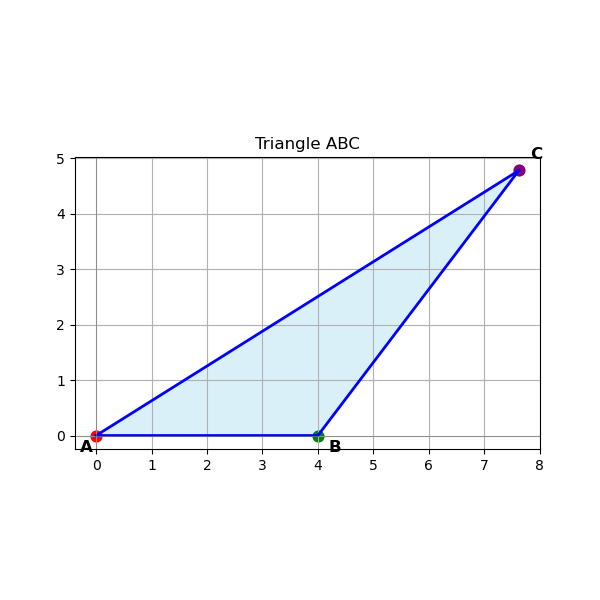
\includegraphics[width=\columnwidth, height=0.8\textheight, keepaspectratio]{figs/Figure_5.png}     

\end{document}